%evaluation.tex

\chapter{Evaluation}
\label{chapter:eva}

Was kann ich mit meinem Modell?

Simulation von Peaks die ideal-gaußförmig sind oder tailing aufweisen

Grenzen des Modells:
Minimalbreite kann nicht unterschritten werden

Formel zur Umrechnung von Peakdaten in Parameter, oder falls das nicht drin ist, zumindest Zusammenhänge, dazu zb Plots von drei festen Parametern
Evtl Tabelle mit exemplarischen Daten, anhand derer weitere gewünschte Peaks angenähert werden können?

3a modell liefert tailing, welches bei 3b nicht gefunden wurde (vielleicht einfach nur die falschen parameter ausprobiert?)
\todo{Mit 3s ist ab jetzt immer 3a gemeint, das andere wurde nicht genauer untersucht}

\section{Relevanter Parameterbereich / relevante Peaks}

\todo{Strukur: erst komplett 2p dann 3s, wegen referenz auf schiefe bei 2p in den params für 3s}

\subsection{2-Parameter Modell}


\subsection{3-Zustände Modell}
\todo{Wo erwähnen, dass nach 240 sec Schluss ist?}


Die wenigen Peaks, die beim 2-Parameter Modell Schiefe aufweisen dienen als Grundlage für eine sinnvolle Parametereinschränkung für $p_{ml}$ und $p_{ll}$. Dabei war zu beobachten, dass die Teilchen nur selten in den stationären Zustand eintreten, dafür aber sehr lange dort verweilen. Um diesen Effekt nachzuahmen, muss $p_{ml}$ dementsprechend sehr klein im Vergleich zu pma und $p_{mm}$ sein. $p_{ll}$ muss dafür sehr groß sein, deutlich größer als paa

In der experimentellen Phase der Arbeit wurden zunächst im gesamten Parameterraum $[0;1]^3$ einige Simulationen durchgeführt, um herauszufinden, in welchen Bereichen sich Peaks ergeben. 
Durch die Beschränkung des Spektrums auf $240$ Sekunden scheiden schon viele Parameterkombinationen aus, welche spätere Peaks erzeugen würden. Das betrifft insbesondere diejenigen Kombinationen, die eine geringe Wahrscheinlichkeit haben, mobil zu bleiben oder zu werden, dafür aber mit einer sehr hohen Wahrscheinlichkeit stationär werden oder bleiben. 
% Für die Schiefe soll es zunächst keine Beschränkungen geben, TODO (gibt es ne sinnvolle Obergrenze, Optik mit Werten vergleichen)
Typischerweise sind Peaks zu Beginn des Spektrums eher schmal, spätere Peaks können breiter werden. Generell lässt sich sagen, dass der IQR eines Peaks geringer sein sollte, als sein Maximalzeitpunkt. Darüber hinaus wurde eine maximale Peakbreite von 10+0.2*maxzeitpunkt TODO festgelegt. Peaks mit höherem IQR sind in einem Spektrum kaum noch als Peaks zu erkennen.
Sehr breite Peaks sind auch nur dann als Peak zu erkennen, wenn sie sehr schief sind.
Für die Schiefe gilt, dass ein Tailing ab einem IQK von 0.2 gut zu erkennen ist. Werte bis 0.4 treten meist bei schiefen Peaks auf, die auch optisch einem realistischen Peak ähneln. Darüber hinaus haben die Peaks oft ein sehr langes Tailing, welches teilweise auch über die Maximalzeit hinausragt. Dieses ist jedoch auf einem so niedrigen Niveau, dass es in einem Spektrum mit Rauschen wahrscheinlich unter gehen würde.
\todo{bewertende aussagen weglassen, habe ja keine vergleichsdaten}
Dadurch ergeben sich folgende Einschränkungen für die verschiedenen Parameter:
\begin{itemize}
 \item $p_{mm}$: keine generellen Einschränkungen, es wurden für Werte im Intervall $[0,005; 0,99]$ Peaks gefunden. Bei noch kleineren Werten TODO bei größeren Werten TODO
 \item $p_{ml}$: sinnvolle Werte liegen im Bereich $[0,00001; 0,001]$. Bei kleineren Werten ergeben sich auch Peaks, die jedoch kein oder fast kein Tailing mehr aufweisen, sodass auch auf das zwei-Parameter-Modell zurückgegriffen werden kann. Bei größeren Werten verweilen die Teilchen so lange im gelösten Zustand, dass die Peaks extrem breit werden, insbesondere, wenn der Parameter $p_{ll}$ auch sehr groß gewählt wurde.
 \item $p_{aa}$: für diesen Parameter wurde der das Intervall auf $[0.997, 0.9996]$ beschränkt. Kleinere Werte sorgen für extrem frühe Peaks. Diese könnten zwar berücksichtigt werden, unterscheiden sich jedoch kaum voneinander. Bei größeren Werten werden die Peaks meist zu breit und zu spät. 
 \item $p_{ll}$: sinnvolle Werte liegen im Bereich $[0,9999; 0,999995]$. Kleinere Werte TODO Bei größeren Werten werden die Teilchen so lange im stationären Zustand gehalten, dass die Peaks meist über das Maximum von 240 Sekunden hinausragen oder zu breit werden. Dies gilt insbesondere, wenn für $p_{ml}$ ebenfalls ein großer Wert gewählt wurde. Im oberen Bereich des Intervalls (>0.999995 erzeugen werden hier Peaks erzeugt, die eine sehr große Schiefe aufweisen, wo der Tail jedoch (wahrscheinlich) im Rauschen verschwindet. Mit den aktuellen Maßen lässt sich das kaum zeigen, wird jedoch beim Blick auf einen geplotteten Peak sofort klar.
\end{itemize}

In allen Fällen gilt jedoch, dass auch jeweils die Kombination der Parameter berücksichtigt werden muss, insbesondere, wenn ein Parameter am Rand des jeweils angegebenen Intervalls liegt, kommt es häufig vor, dass er nur in einigen wenigen Kombinationen für realistische Peaks sorgt.
Beispiele: TODO: ein paar Kombis nennen, die grenzwertig, bzw drüber hinaus sind.



\section{Einfluss der verschiedenen Parameter auf Peaks}

In den meisten Fällen kann ein deutlicher Zusammenhang zwischen den Parametern und Peakdaten beobachtet werden, diese seien im Folgenden aufgeführt.

\subsection{2-Parameter Modell} 

Sowohl Zeitpunkt als auch Breite der Peaks hängen von ps und pm ab.
Nur in einem sehr kleinen Bereich, bei dem die Peaks ihren Maximalzeitpunkt bei etwa TODO haben, tritt überhaupt Schiefe auf. 


\subsection{3-Zustände Modell}
Bei diesem Modell ergeben sich durch die größere Anzahl an Parametern, komplexere Zusammenhänge zwischen den Parametern und den Peakdaten. Teilweise hängt die Stärke des Einflusses eines Parameters auf ein Peakcharakteristikum vom Wert eines anderen Parameters ab. Das heißt, der Einfluss eines Parameters auf die Peaks kann größer oder kleiner sein, abhängig davon, ob ein anderer Parameter eher im oberen oder unteren Bereich seines oben angegebenen Intervalls liegt.
Zunächst können jedoch folgenden Zusammenhänge gefunden werden:

Für den Maximalzeitpunkt des Peaks sowie seine Breite gilt, dass beide größer werden, wenn die Parameter $p_{ml}$, $p_{aa}$ und $p_{ll}$ größer werden oder $p_{mm}$ kleiner wird. 
Die Schiefe steigt mit fallendem $p_{aa}$ und in den meisten Fällen mit steigendem $p_{mm}$. Für $p_{ml}$, $p_{ll}$ und in wenigen Fällen auch $p_{mm}$ ist zu beobachten, dass bei größer werdenden Parametern die Schiefe zunächst auch ansteigt, ab einem gewissen Wert jedoch sinkt.

Insgesamt gilt, dass die Einflüsse auf Zeitpunkt und Breite der Peaks weniger komplex sind, als die Einflüsse auf die Schiefe. Das ist auch damit erklärbar, dass für Zeitpunkt und Breite eigentlich nur die zwei Parameter des einfachen Modells nötig sind und die Aufsplittung des stationären Zustands daran nicht viel ändert. Die Schiefe jedoch hängt immer von mehreren Parametern und deren Kombination ab.

%TODO: Das folgende ist zwar interssant, aber eher so eine Zusammenfassung
%Da bei einem Wert von $0$ für $p_{ml}$ effektiv das zwei-Parameter-Modell zum Einsatz kommt, ist hier fast nie Schiefe zu beobachten, außerdem hat der Parameter $p_{ll}$ keinen Einfluss. 
% 
% $p_{aa}$ hat einen stärkeren Einfluss auf den Zeitpunkt als $p_{ll}$ und $p_{ml}$. Dieser wird noch stärker, wenn $p_{mm}$ klein ist
% 
% $p_{mm}$ hat einen großen Einfluss auf den Zeitpunkt und nur einen minimalen Einfluss auf die Breite.
% 
% $p_{ml}$ und $p_{ll}$ haben zunächst beide einen proportionalen Einfluss auf die Schiefe. Erst, wenn beide sehr groß sind, sinkt die Schiefe wieder (und die Breite steigt extrem an) Das ist wohl dadurch zu erklären, dass sich nicht mehr genügend Teilchen im mobil-adsorbierten System befinden, wodurch ein normaler Peak entstehen kann. Statt dass die Lösung Schiefe an diesem einfachen Peak verursacht, sorgt sie nunmehr für Breite
% 
% Tailing/Schiefe entsteht immer da, wo nur wenige Teilchen langsamer sind, als die große Masse. Sind viele Teilchen lange stationär, werden die Peaks statt dessen breit. Der Maximalzeitpunkt ist hauptsächlich durch die Durchschnittsgeschwindigkeit der Teilchen bestimmt, sind sie hauptsächlich mobil, entstehen frühe Peaks, sind sie oft und lange stationär, wandern die Peaks nach hinten.

Im Folgenden ist für jeden der vier Parameter eine detaillierte Übersicht gegeben welche Eigenschaften der Peaks er in Abhängigkeit anderer Parameter beeinflusst.

\paragraph*{Einfluss des Parameters $p_{mm}$}

\begin{figure}[H]
\begin{subfigure}{0.6\textwidth}
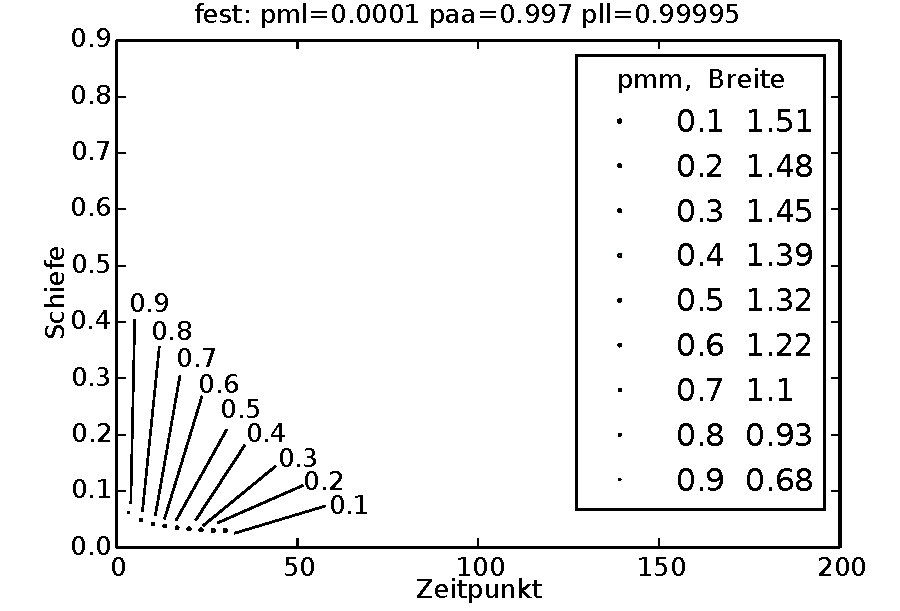
\includegraphics[width=\textwidth]{bilder/pmm/3fest_p_00001_0997_099995}
\caption{$p_{aa}$ klein}
\end{subfigure}

\begin{subfigure}{0.6\textwidth}
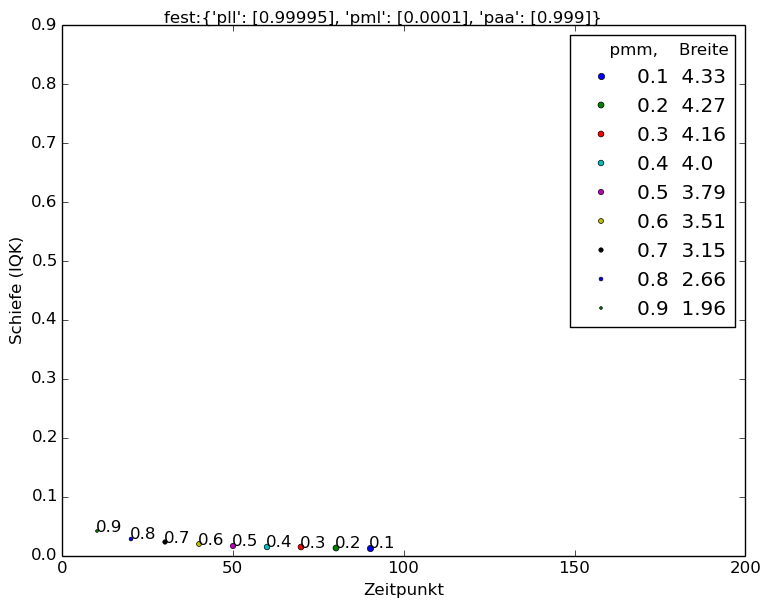
\includegraphics[width=\textwidth]{bilder/pmm/3fest_p_00001_0999_099995}
\caption{$p_{aa}$ mittel}
\end{subfigure}

\begin{subfigure}{0.6\textwidth}
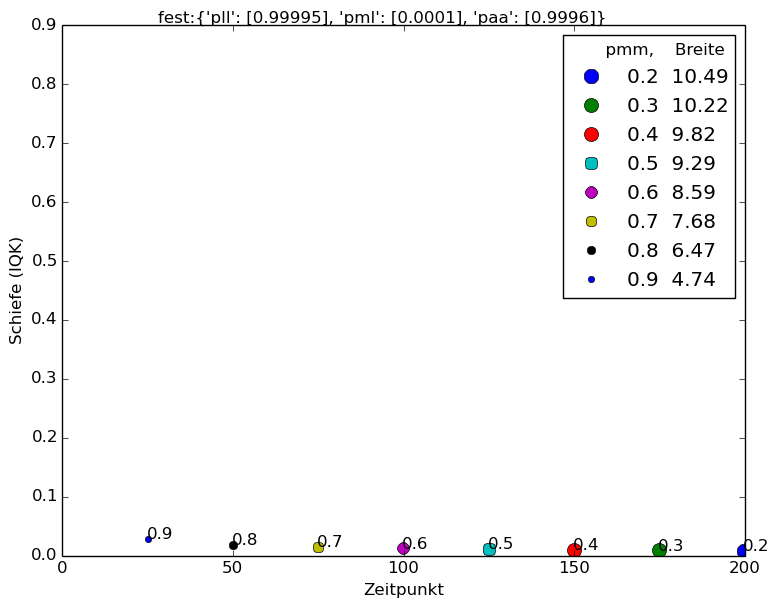
\includegraphics[width=\textwidth]{bilder/pmm/3fest_p_00001_09996_099995}
\caption{$p_{aa}$ groß}
\end{subfigure}
\caption{Der Einfluss von $p_{mm}$ auf die Peaks abhängig von $p_{aa}$}
\label{einfluss_pmm_1}
\end{figure}

\todo{Plotbeschriftung (Titel), Plots nachbearbeiten, Größe der Plots}

Wie in Abbildung \ref{einfluss_pmm_1} zu sehen, ist der Einfluss von $p_{mm}$ auf den Zeitpunkt von $p_{aa}$ abhängig: Je größer $p_{aa}$ ist, desto stärker wird der Zeitpunkt von $p_{mm}$ beeinflusst. Wenn $p_{mm}$ und $p_{aa}$ klein sind, entstehen nur Peaks zu Beginn des Spektrums, unabhängig von $p_{ml}$ oder $p_{ll}$.

Der Einfluss von $p_{mm}$ auf die Breite ebenfalls von paa abhängig. Bei größerem $p_{aa}$ steigt dieser Einfluss etwas, wie ebenfalls in Abbildung \ref{einfluss_pmm_1} zu erkennen ist. Dieser Zusammenhang ergibt sich daraus, dass sich in diesem Fall auch der Maximalzeitpunkt nach hinten verschiebt und spätere Peaks generell breiter sind, als frühe Peaks.

\todo{Noch mal den kleinen Bereich untersuchen, wo die Schiefe negativ beeinflusst wird. Das ist ein Bereich, in dem die Peaks zwar sehr früh, aber dafür fast zu breit sind. Vielleicht hängt das damit zusammen? siehe: $p_{mm}$0.001 0.998 0.99999}

% \begin{figure}[H]
% \begin{subfigure}[t]{0.5\textwidth}
% \includegraphics[width=\textwidth]{bilder/}
% \caption{$p_{aa}$ groß und $p_{ml}$ groß}
% \end{subfigure}
% \begin{subfigure}[t]{0.5\textwidth}
% \includegraphics[width=\textwidth]{bilder/}
% \caption{$p_{aa}$ groß und $p_{ml}$ klein}
% \end{subfigure}
% \vspace*{7mm}
% \begin{subfigure}[b]{0.5\textwidth}
% \includegraphics[width=\textwidth]{bilder/}
% \caption{$p_{aa}$ klein und $p_{ml}$ groß}
% \end{subfigure}
% \begin{subfigure}[b]{0.5\textwidth}
% \includegraphics[width=\textwidth]{bilder/}
% \caption{$p_{aa}$ klein und $p_{ml}$ klein}
% \end{subfigure}
% \caption{Der Einfluss von $p_{mm}$ auf die Schiefe abhängig von $p_{aa}$, $p_{ml}$ und $p_{ll}$}
% \label{einfluss_pmm_2}
% \end{figure}



Außer in einem sehr kleinen Parameterbereich, steigt die Schiefe mit steigendem $p_{mm}$. Dieser Einfluss hängt noch von $p_{aa}$ ab, bei kleinem $p_{aa}$ hat $p_{mm}$ einen größeren Einfluss auf die Schiefe. Hängt aber auch von pml/pll ab! 

\begin{figure}[H]
\begin{subfigure}{0.6\textwidth}
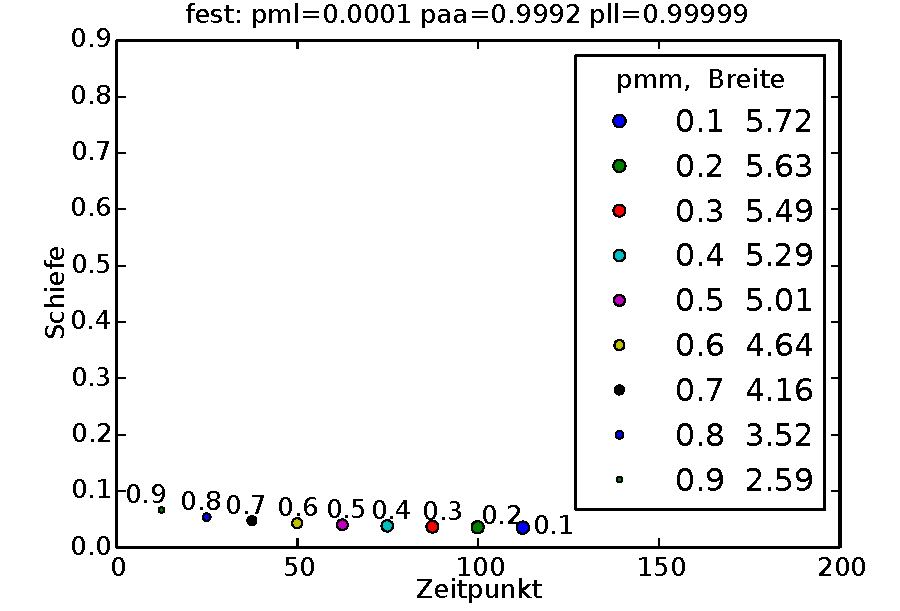
\includegraphics[width=\textwidth]{bilder/pmm/3fest_p_00001_09992_099999}
\caption{$p_{ml}$ klein}
\end{subfigure}

\begin{subfigure}{0.6\textwidth}
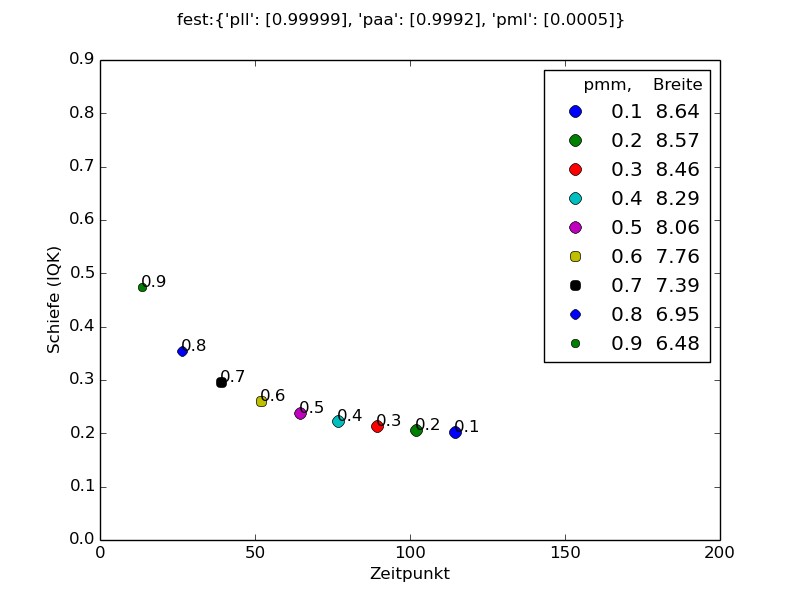
\includegraphics[width=\textwidth]{bilder/pmm/3fest_p_00005_09992_099999}
\caption{$p_{ml}$ mittel}
\end{subfigure}

\begin{subfigure}{0.6\textwidth}
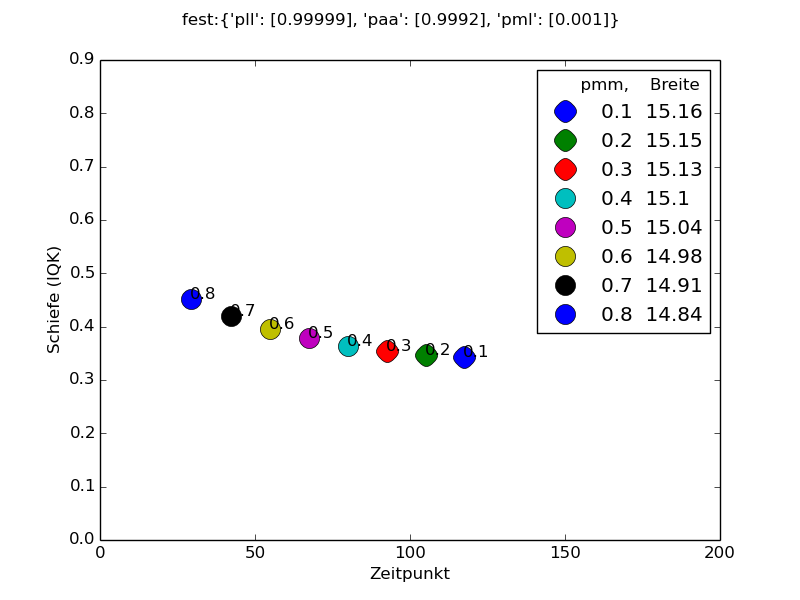
\includegraphics[width=\textwidth]{bilder/pmm/3fest_p_0001_09992_099999}
\caption{$p_{ml}$ groß}
\end{subfigure}
\caption{Der Einfluss von $p_{mm}$ auf die Peaks abhängig von $p_{ml}$}
\label{einfluss_pmm_2}
\end{figure}

Einfluss von $p_{mm}$ auf die Schiefe ist am größten bei mittlerem $p_{ml}$ und (etwa im Intervall $[0,0001, 0,0005]$) und mittlerem pll (etwa bei $[0,99995-0,99999]$). Dieser Zusammenhang ist für pml in Abbildung \ref{einfluss_pmm_2} dargestellt.
Zusätzlich wird der Einfluss von $p_{ml}$ und $p_{ll}$ auf die Abhängigkeit der Schiefe von pmm größer, wenn paa klein ist.

Dieser Zusammenhang kann wie folgt erklärt werden: $p_{ml}$ und $p_{ll}$ verursachen gemeinsam das Tailing. Dieser Effekt kann sich bei großem $p_{mm}$ besser zeigen. Dann sind die Teilchen im Durchschnitt schneller. Ein kleiner Wert für paa sorgt ebenfalls für eine höhere Durchschnittsgeschwindigkeit. Dadurch geraten im Gesamtverlauf der Säulendurchquerung Teilchen seltener in den gelösten Zustand, wo sie das Tailing erzeugen. Bei durchschnittlich langsameren Teilchen lösen sich die Teilchen zu häufig und statt Schiefe entsteht wiederum Breite.
Ist $p_{aa}$ jedoch zu klein und $p_{ll}$ zu groß entstehen Peaks, die einen extrem großen Interquartilskoeffizienten haben. Allerdings ist der Tail so flach, dass er in einem Gesamtchomatogramm wohl eher im Rauschen untergehen würde.

% TODO: Gehört ans Ende: Ist $p_{ml}$ zu klein, hat der gelöste Zustand fast keinen Einfluss und es entsteht unabhängig von $p_{mm}$ kaum Schiefe. Gleiches gilt für pll, ist es zu klein, verweilen die Teilchen nicht lange genug, um Tailing zu verursachen.
% Wenn pml und pll jedoch zu groß werden, 
%  ist $p_{ml}$ zu groß, werden die Peaks wieder nur breit, aber nicht so schiefa die Teilchen, die nicht in den gelösten Zustand kommen, sich recht schnell fortbewegen (daher auch besonders bei kleinem $p_{aa}$ zu beobachten) und dadurch nur wenige Teilchen langsamer sind und dadurch den Tail verursachen. Ist paa kleiner, lösen sich die Teilchen häufiger und statt der schiefen entstehen breite Peaks.


\paragraph*{Einfluss des Parameters pml}

\begin{figure}
\begin{subfigure}[t]{0.5\textwidth}
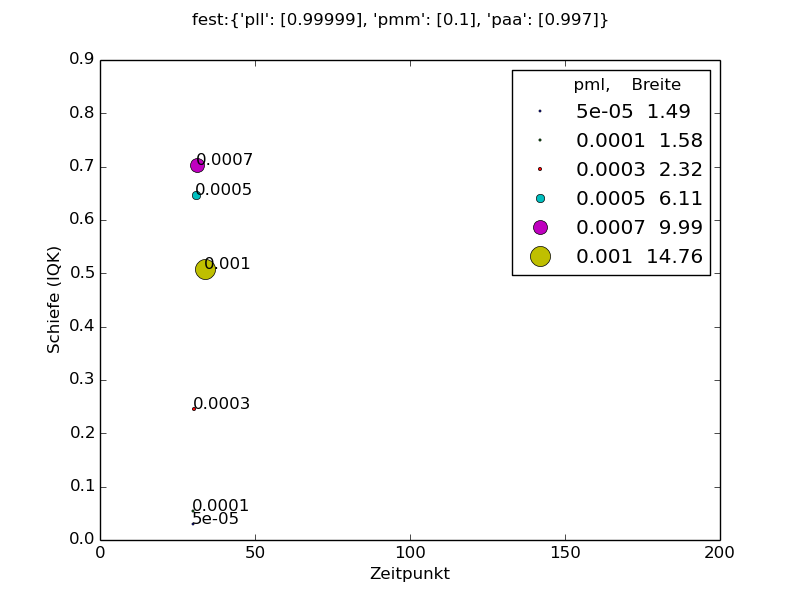
\includegraphics[width=\textwidth]{bilder/pml/pml_01_p_0997_099999}
\caption{$p_{ll}$ sehr groß}
\label{einfluss_pml_pll++}
\end{subfigure}
\begin{subfigure}[t]{0.5\textwidth}
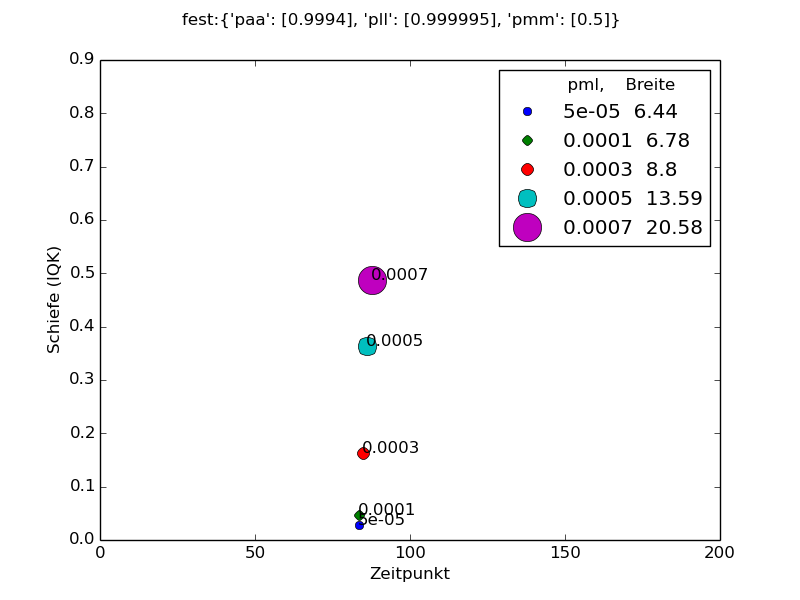
\includegraphics[width=\textwidth]{bilder/pml/pml_05_p_09994_0999995}
\caption{$p_{ll}$ groß}
\label{einfluss_pml_pll+}
\end{subfigure}
\vspace*{7mm}
\begin{subfigure}[b]{0.5\textwidth}
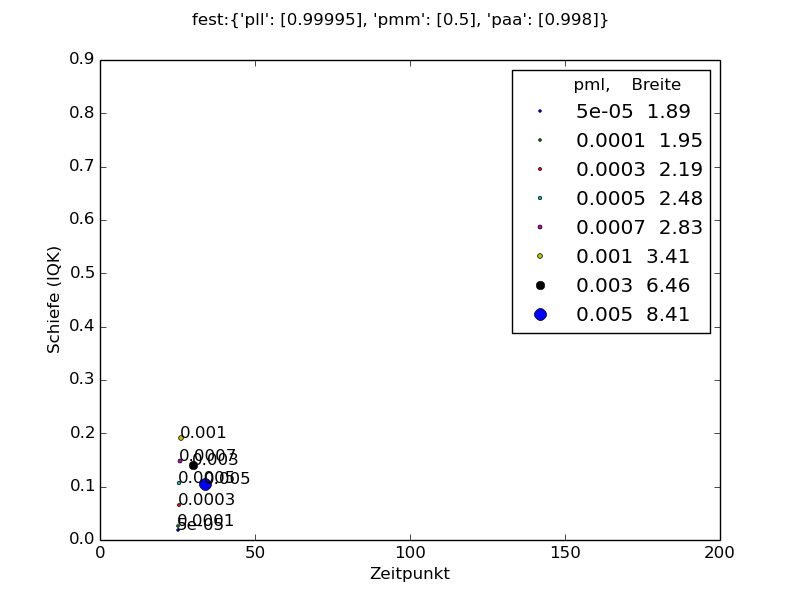
\includegraphics[width=\textwidth]{bilder/pml/pml_05_p_0998_099995}
\caption{$p_{ll}$ klein}
\label{einfluss_pml_pll-}
\end{subfigure}
\begin{subfigure}[b]{0.5\textwidth}
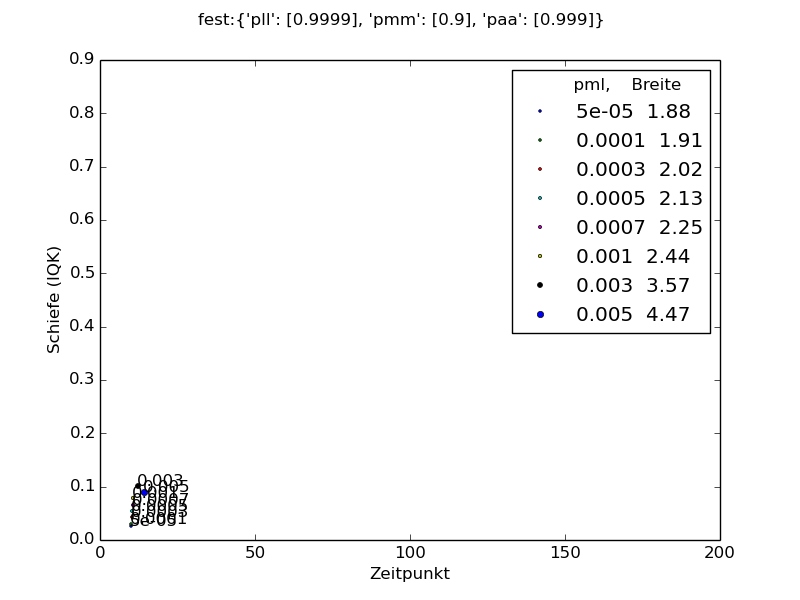
\includegraphics[width=\textwidth]{bilder/pml/pml_09_p_0999_09999}
\caption{$p_{ll}$ sehr klein}
\label{einfluss_pml_pll--}
\end{subfigure}
\caption{Der Einfluss von $p_{ml}$ auf die Schiefe und Breite abhängig von $p_{ll}$}
\label{einfluss_pml_1}
\end{figure}

Der Einfluss von $p_{ml}$ auf die Peakdaten ist in den Abbildungen \ref{einfluss_pml_1} und \ref{einfluss_pml_2} gezeigt. Schiefe und Breite sind häufig deutlich von $p_{ml}$ beeinflusst, der Zeitpunkt hingegen kaum. Allenfalls sehr große Werte für $p_{ml}$ sorgen für einen erkennbar höheren Zeitpunkt, dann aber auch für deutlich mehr Breite und weniger Schiefe.

\begin{figure}
\begin{subfigure}[t]{0.5\textwidth}
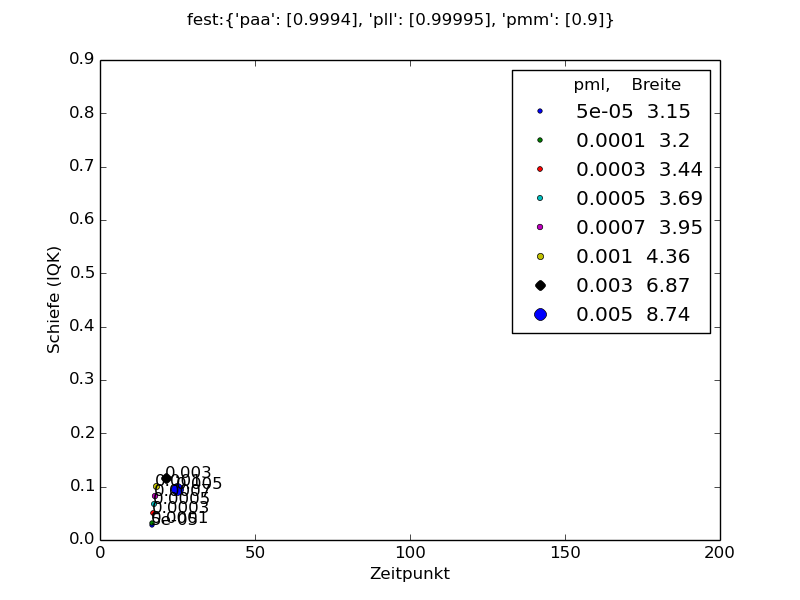
\includegraphics[width=\textwidth]{bilder/pml/pml_09_p_09994_099995}
\caption{$p_{mm}$ groß, $p_{aa}$ groß}
\end{subfigure}
\begin{subfigure}[t]{0.5\textwidth}
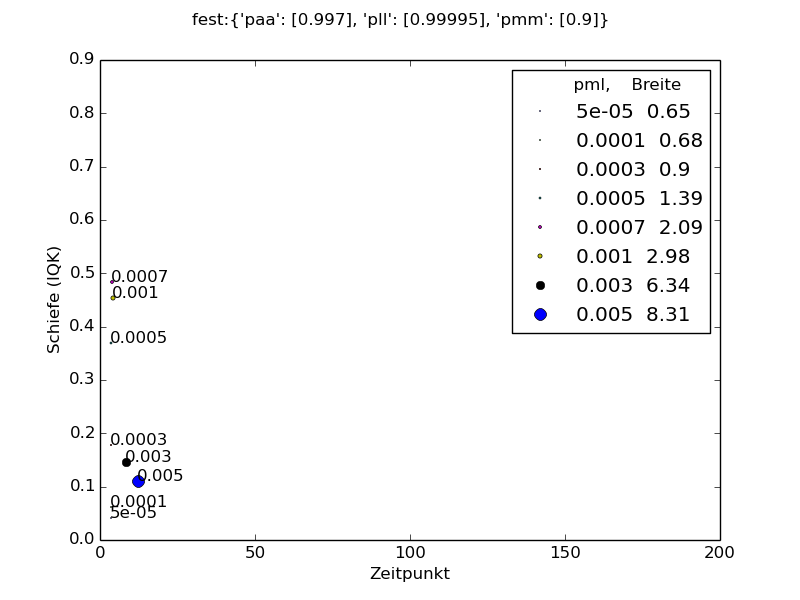
\includegraphics[width=\textwidth]{bilder/pml/pml_09_p_0997_099995}
\caption{$p_{mm}$ groß, $p_{aa}$ klein}
\end{subfigure}
\vspace*{7mm}
\begin{subfigure}[b]{0.5\textwidth}
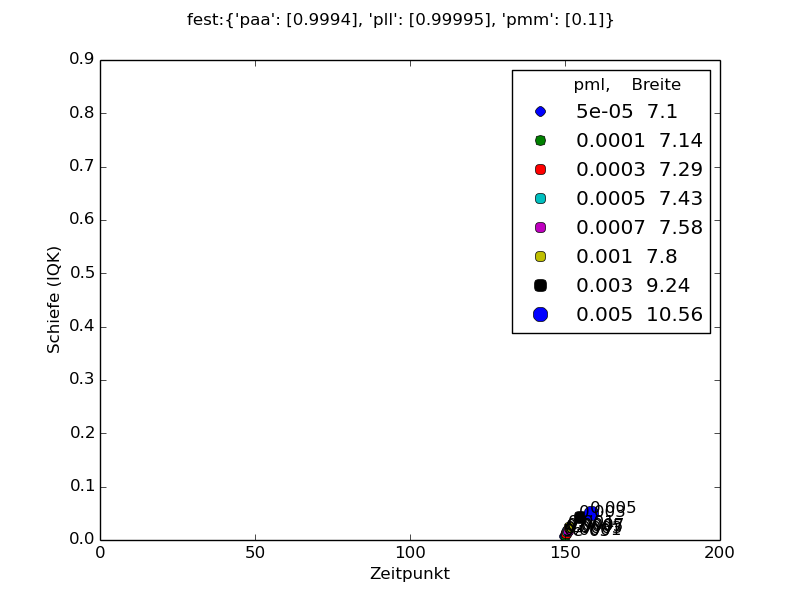
\includegraphics[width=\textwidth]{bilder/pml/pml_01_p_09994_099995}
\caption{$p_{mm}$ klein, $p_{aa}$ groß}
\end{subfigure}
\begin{subfigure}[b]{0.5\textwidth}
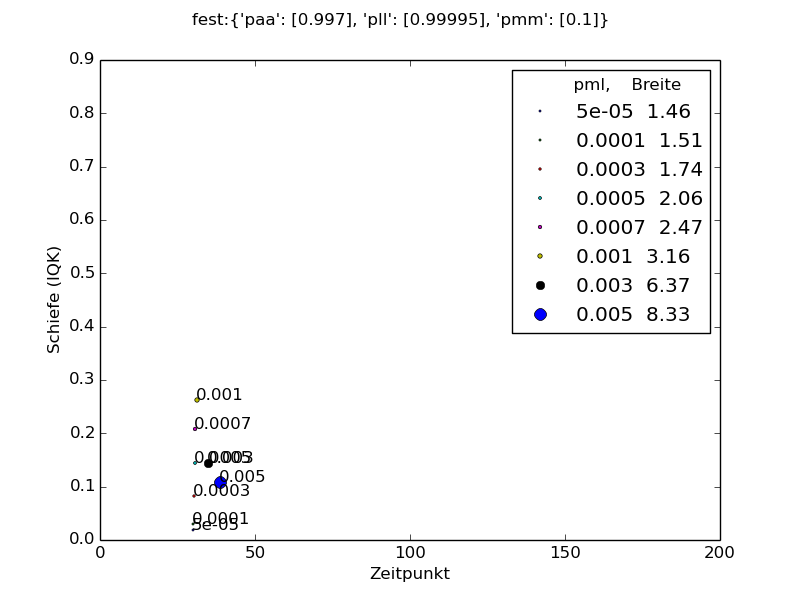
\includegraphics[width=\textwidth]{bilder/pml/pml_01_p_0997_099995}
\caption{$p_{mm}$ klein, $p_{aa}$ klein}
\end{subfigure}
\caption{Der Einfluss von $p_{ml}$ auf die Schiefe und Breite abhängig von $p_{mm}$ und paa}
\label{einfluss_pml_2}
\end{figure}

Auf die Schiefe und Breite ist der Einfluss von $p_{ml}$ sehr groß, wenn auch $p_{ll}$ groß ist, wie in Abbildung \ref{einfluss_pml_1} zu erkennen. Hier sind $p_{mm}$ und $p_{aa}$ auf allen vier Plots gleich gewählt, nur $p_{ll}$ nimmt von \ref{einfluss_pml_pll++} nach \ref{einfluss_pml_pll--} ab und damit schwindet auch der Einfluss von $p_{ml}$ auf Schiefe und Breite.

Wie in Abbildung \ref{einfluss_pml_2} gezeigt, spielen auch $p_{mm}$ und $p_{aa}$ für den Einfluss von $p_{ml}$ auf Schiefe und Breite eine Rolle. Hier ist $p_{ll}$ in allen vier Plots konstant, $p_{mm}$ und $p_{aa}$ werden variiert. Zu erkennen ist, dass bei kleinem paa, der Einfluss von $p_{ml}$ auf Schiefe und Breite größer wird, ist $p_{mm}$ jedoch klein, wird auch der Einfluss von $p_{ml}$ kleiner.


\paragraph*{Einfluss des Parameters paa}

\begin{figure}[H]
\begin{subfigure}[t]{0.5\textwidth}
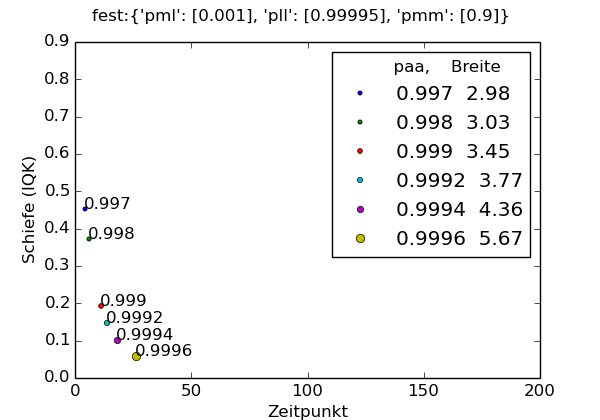
\includegraphics[width=\textwidth]{bilder/paa/3fest_09_0001_p_099995}
\caption{$p_{mm}$ und $p_{ml}$ groß}
\end{subfigure}
\begin{subfigure}[t]{0.5\textwidth}
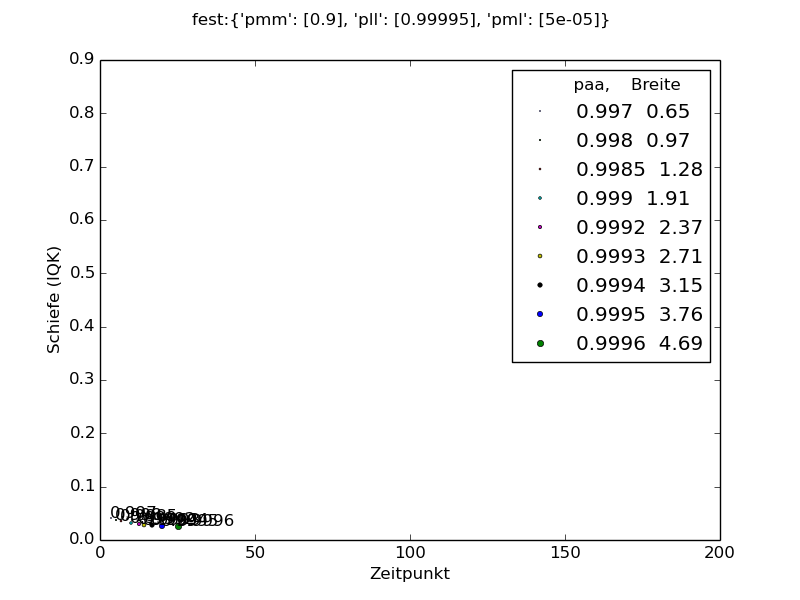
\includegraphics[width=\textwidth]{bilder/paa/3fest_09_5e-05_p_099995}
\caption{$p_{mm}$ groß und $p_{ml}$ klein}
\end{subfigure}
\vspace*{7mm}
\begin{subfigure}[b]{0.5\textwidth}
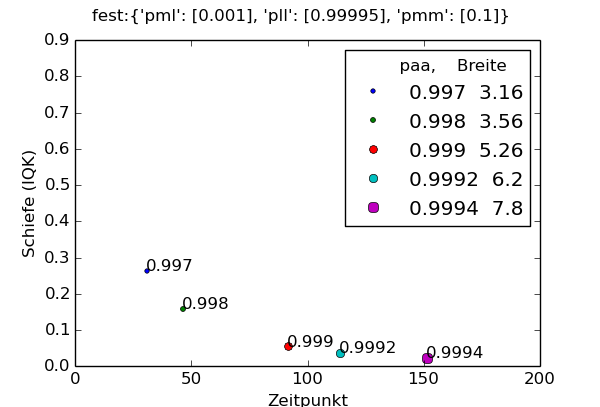
\includegraphics[width=\textwidth]{bilder/paa/3fest_01_0001_p_099995}
\caption{$p_{mm}$ klein und $p_{ml}$ groß}
\end{subfigure}
\begin{subfigure}[b]{0.5\textwidth}
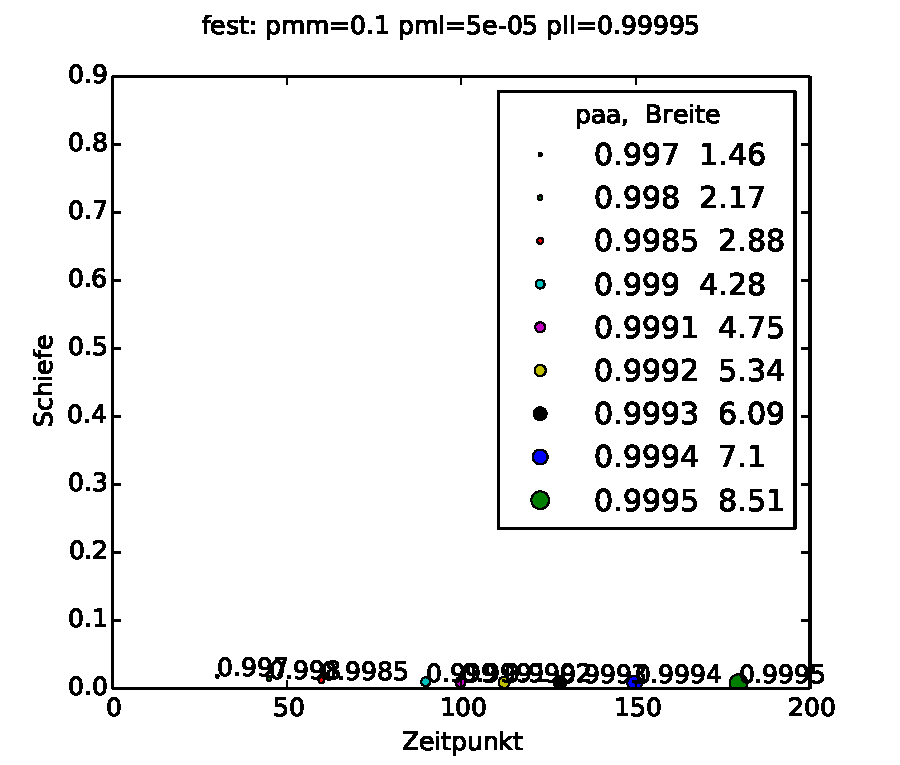
\includegraphics[width=\textwidth]{bilder/paa/3fest_01_5e-05_p_099995}
\caption{$p_{mm}$ und $p_{ml}$ klein}
\end{subfigure}
\caption{Der Einfluss von $p_{aa}$ auf die Peaks abhängig von $p_{mm}$ und $p_{ml}$}
\label{einfluss_paa}
\end{figure}

In Abbildung \ref{einfluss_paa} ist beispielhaft der Einfluss von Parameter $p_{aa}$ auf die Peaks gezeigt. Der Einfluss von $p_{aa}$ auf den Zeitpunkt wird mit steigendem $p_{mm}$ immer kleiner und reicht dadurch von minimalem Einfluss und recht frühen Peaks bei jeder Wahl von $p_{aa}$ bis zu sehr großem Einfluss und Peaks, die je nach $p_{aa}$ über das ganze Spektrum verteilt sind. Damit hat $p_{aa}$ einen ähnlichen Einfluss wie $p_{mm}$.

$p_{aa}$ hat nur dann einen relevanten Einfluss auf die Schiefe, wenn $p_{ml}$ mittelgroß ist. Bei zu großem $p_{ml}$ werden Peaks statt dessen wieder nur breit und bei zu kleinem $p_{ml}$ hat $p_{aa}$ kaum Einfluss auf die schiefe. 

Der Einfluss auf die Breite ist mäßig und wird größer, wenn $p_{ml}$ und $p_{ll}$ klein sind.

TODO: $p_{ll}$ verändert auch den Einfluss von paa, das hängt aber von $p_{mm}$ und $p_{ml}$ ab.


\paragraph*{Einfluss des Parameters pll}

Der Einfluss von $p_{ll}$ auf den Zeitpunkt ist ähnlich wie bei pml nur minimal.
Wenn pml nicht zu klein ist, hat pll einen großen Einfluss auf Schiefe und Breite

\section{Grenzen der Modelle}

Wie bereits erwähnt, ist es mit dem 2-Parameter Modell nur eingeschränkt möglich, Tailing zu erzeugen. Insbesondere  dieses nicht zu den späteren Zeitpunkten im Chromatogramm auf. Dieses Problem konnte, wie gezeigt, mit dem 3-Zustände Modell behoben werden. 
Eine weitere Grenze ist jedoch die Minimalbreite der erzeugten Peaks. Damit ist par, dass mit zunehmender Zeit die Minimalbreite der Peaks, die an diesem Zeitpunkt ihr Maximum haben, ansteigt. 
\todo{Plot der Zeit/Breiten-Verhältnisse, Gesamtübersicht, sowie einzelverläufe mit sichbarerm erreichen der parametergrenzen (0)}
Dieses Problem kann mit dem 3-Zustände Modell nicht gelöst werden, da die Peaks durch Hinzunahme eines weiteren stationären Zustandes höchstens breiter werden. 

\section{Laufzeiten}
